\documentclass{article}
\usepackage{hyperref}
\usepackage{graphicx}
\usepackage{siunitx}
\begin{document}
\section{DECAM Information}
From the DECam Imager Handbook: \newline
\begin{figure}[hbt!]
    \centering
    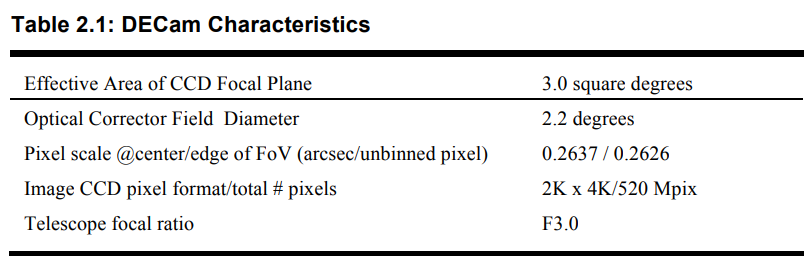
\includegraphics[width=0.5\linewidth]{Decam Characteristics.png}
    \caption{DECam Characteristics}
    \label{fig:enter-label}
\end{figure}
DECam has a three square degree field of view (2.2 degrees wide). It images at a resolution of 0.263 arcseconds per pixel. In particular, 0.2637 arcsec/pixel (center), 0.2626 arcsec/pixel (edge).  0.2637/0.2626 (arcsec/unbinned pixel). S Large focal plane array with a close to circular array of 62 CCDs and a total of 520 million pixels. 
\newline 
CCD Array Characteristics:
\newline
Array Dimensions: 
    Axis 1: 2048 pixels
    Axis 2: 4096 pixels
\newline
Pixel Size: \SI{15}{\micro\metre}


We are looking to use \textbf{resampled} images that have a zero-point associated with them. In the astro data archive, this corresponds to files with the process type (\texttt{proc\_type}) of \texttt{resampled}, and the presence of the \texttt{MAGZERO} and\/or \texttt{MAGZPT} fields.

\textbf{Maggie:} Linear flux units, where an object with an AB magnitude of 0 has a flux of 1.0 maggie. A convenient unit is the nanomaggie: a flux of 1 nanomaggie corresponds to an AB magnitude of 22.5.

\texttt{MAGZERO} data field: The (astronomical) magnitude corresponding to a single photon count in the image. This is located in the \textit{Extension} headers of the FITS files, present in Level 2 data products (single, reduced exposures). (From the DECam data handbook)\\

\section{Declination Range of the 2.3m Telescope}
\href{https://www.cambridge.org/core/journals/publications-of-the-astronomical-society-of-australia/article/anu-wifes-supernova-programme-awsnap/1DF292200162D34D6E5A268CE18C3653} {Physical Pointing Limit of the 2.3m}
\begin{figure}[hbt!]
    \centering
    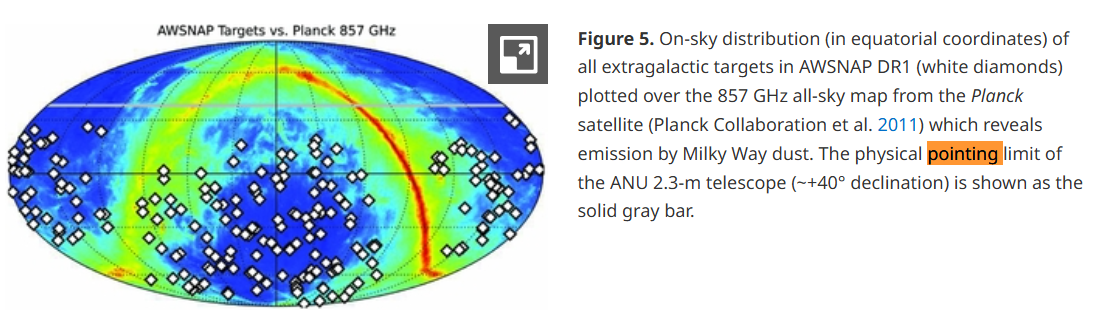
\includegraphics[width=0.5\linewidth]{image.png}
    \caption{Enter Caption}
    \label{fig:enter-label}
\end{figure}

\href{https://datalab.noirlab.edu/skymapper.php#:~:text=SMSS%20published%20its%20Fourth%20Data,observed%20up%20to%20%2B28%C2%B0.} {Sky Mapper Coverage}

Notes from Proposal\\
go for volume, ample padding in exclusion zones rather than extreme accuracy (we are ok with generating less positions that are definitely good

  \section{link dump}

  \href{https://github.com/cyb0rb/WiFeS_Catalog}{github repo}
  
  \href{https://sep.readthedocs.io/en/v1.1.x/tutorial.html}{source extractor tutorial}

  \href{https://github.com/astro-datalab/notebooks-latest/blob/aa7e2954d538632a5f0a26665c91906ca2c9cfbc/04_HowTos/SiaService/How_to_use_the_Simple_Image_Access_service.ipynb}{SIA querying with the astro datalab}

\subsection{DECam}
  \href{https://astroarchive.noirlab.edu/api/docs/}{NOIRLab astro data archive}

  \href{https://github.com/NOAO/nat-nb/blob/master/sia.ipynb}{data archive query example notebook}

  \href{https://www.darkenergysurvey.org/the-des-project/data-access/}{DES project data access}

  \href{https://noirlab.edu/science/sites/default/files/media/archives/documents/scidoc0436.pdf}{DECam imager data handbook}
  
  \href{https://noirlab.edu/science/programs/ctio/instruments/Dark-Energy-Camera}{NOIRLab DECam information page} (has more links)
  
  \href{https://des.ncsa.illinois.edu/releases/other}{DES Data Management}

  \href{https://aus01.safelinks.protection.outlook.com/?url=https}{2.3m projects}


\section{Word Dump}

As a stretch goal, we may also then apply our software to generate a full catalogue of sky positions, ideally covering as much of the southern sky within the reach of the 2.3m as possible. This would involve iterating our software through the DESI Legacy Imaging Survey database which is a combintaion of the DECam Legacy Survey, the Beijing-Arizona Sky Survey, and the Mayall z-band Legacy Survey, finding all associated dark regions for targets in the entire sky.

The decision to start simple by just trying to complete the querying, source extractor and dark sky identification process for a single image was made taking into consideration potential contingencies throughout the internship and thus, if a final software and catalogue can not be produced for a range of queried images, it can at least be done for one which can be expanded upon.

\section{Querying from Monday 3/02/25}
\subsection{Range of RA and DEC}
Range of the 2.3m Telescope is across all RA and for DEC$<$30 degrees. 
Thus, only images from the Legacy Survey dr10 $<$30 degrees in declination will be considered.

\section{Threshold Calculation}
The threshold value (a) for the source extractor was found using, \begin{equation} a=f/\sigma_{rms} \end{equation}
where $\sigma_{rms}$ is the background noise level or the global background RMS of the image and f is the pixel flux value in nanomaggies corresponding to a given limiting AB magnitude and zero point. For reference, an object with an AB magnitude of 22.5 has a flux of 1 nanomaggie [Data Release Description Reference].\\
\\Firstly, the background noise level or the global background RMS of the image ($\sigma_{rms}$) was extracted using bkg= sep.Background() followed by bkg.globalrms(). The flux value (f) was then calculated as,  \begin{equation} 
f=10^{(z-m)/2.5}
\end{equation} 
Where m is the limiting (AB) magnitude (21 for this catalogue) and z is the zero point (AB) magnitude of the image (22.5 for the DR10 stacked images). \\
\\ 
Substituting the two values into Equation 1 gives the threshold pixel value for detection or the value at which a pixel is classed as belonging to an object and thus, will not considered as a potential dark sky position.


 \section{Extras}
Moreover, the zero-point magnitude of the image was extracted from the header using image.header['MAGZERO'] which is 22.5 for the Legacy Survey DR10 images. This equation can then be rearranged to take in the limiting magnitude (21) and give the threshold pixel flux value at which a pixel with a value above that threshold is identified as belonging to an object and cannot be considered for a dark sky position.  \\
The threshold value (a) for the source extractor can be found using, \begin{equation} a=f/\sigma_{rms} \end{equation}
where $\sigma_{ab}$ is the background noise level or the global background RMS of the image and f is the linear flux value in nanomaggies (an object with an AB magnitude 22.5 has a flux of 1 nanomaggie).\\
\\Firstly, the background noise level or the global background RMS of the image ($\sigma_{rms}$) was extracted using bkg= sep.Background() followed by bkg.globalrms(). \\
\\The flux value (f) can then be calculated by rearranging the below equation,  \begin{equation} 
m=z-2.5\times log_{10}(f)
\end{equation} 
Where m is the limiting (AB) magnitude (21 for this catalogue), z is the zero point (AB) magnitude of the image (22.5 for the DR10 stacked images) and f is linear flux measured in nanomaggies (an object with an AB magnitude 22.5 has a flux of 1 nanomaggie) [Data Release Description Reference]. This equation can then be rearranged to take in the limiting magnitude (21) and give the threshold pixel flux value at which a pixel with a value above that threshold is identified as belonging to an object and cannot be considered for a dark sky position.
\end{document}